\documentclass[10pt,a4paper]{article}
\usepackage[a4paper,margin=2cm]{geometry}
\usepackage[sfdefault]{arimo} % Arimo has the same letter widths as Arial (handout: Arial 10pt)
\usepackage[T1]{fontenc}
\usepackage{amsmath,amssymb}
\usepackage{graphicx}
\usepackage{hyperref}
\usepackage{caption}
\usepackage{float}
\usepackage{booktabs}
\usepackage{xcolor}
\usepackage{titlesec}
\usepackage{tabularx}
\usepackage{tikz}
\usetikzlibrary{arrows.meta,fit,positioning}

\newcommand{\todo}[1]{\textcolor{red}{[TODO: #1]}}

\captionsetup{font=small, labelfont=bf, skip=4pt}
\titleformat{\section}{\large\bfseries}{\thesection}{0.6em}{}
\titlespacing*{\section}{0pt}{1.2ex}{0.6ex}
\titleformat{\subsection}{\normalsize\bfseries}{\thesubsection}{0.6em}{}
\titlespacing*{\subsection}{0pt}{0.8ex}{0.3ex}
\titlespacing*{\paragraph}{0pt}{0.6ex}{0.8em}

\begin{document}

\begin{titlepage}
\centering

\includegraphics[width=0.42\textwidth]{figures/ntu_logo.png}\par
\vspace{1.4cm}
{\large SC4001 Neural Networks and Deep Learning\par}
\vspace{0.15cm}
{\normalsize Group Project Report\par}
\vspace{0.9cm}
\rule{\textwidth}{0.8pt}\par
\vspace{0.45cm}
{\LARGE\bfseries AI Image Detection: Which Meta-learners Help\\[2pt] Expert Models Generalise to Unseen Generators?\par}
\vspace{0.3cm}
\rule{\textwidth}{0.8pt}\par
\vspace{0.9cm}
{\large Group 40\par}
\vspace{0.6cm}
{\renewcommand{\arraystretch}{1.5}
\begin{tabular}{@{}p{6cm}p{5cm}@{}}
\toprule
\textbf{Name} & \textbf{Matriculation number} \\
\midrule
Firas Mosbeh & \\
Lída Pavelková & \\
Tim Martin Kausemann & \\
\bottomrule
\end{tabular}\par}
\vspace{1.0cm}
\begin{minipage}{\textwidth}
\small
\textbf{Abstract.} Detectors of AI-generated images are usually trained on a few known generators, and they often fail on images from a generator they have not seen. We ask whether a combination of generator-specific experts does better on a generator that none of the experts has seen. On a 176,000-image subsample of GenImage, we train seven experts per backbone (linear probes on frozen CLIP features and fine-tuned ResNet-50 networks) and compare eight ways of combining them under leave-one-generator-out evaluation, with paired bootstrap intervals. Every combiner beats the best single expert chosen on the known generators by a wide margin (unseen AUROC 0.972 vs 0.908 for CLIP, 0.950 vs 0.806 for ResNet-50). Knowing which expert produced which score never helps, and extra combiner capacity only pays off for the ResNet experts. A single detector trained on all known generators, however, beats every combiner on both backbones (0.975 for CLIP, 0.978 for ResNet-50), by a margin that is small for CLIP and large and consistent for ResNet-50. We argue that this is a limit of the expert scores themselves, not of the combiners.
\end{minipage}
\vfill
{\normalsize November 2026\par}
\end{titlepage}

% Contents page: no page number, and like the cover it does not count towards the 10 pages.
\tableofcontents
\thispagestyle{empty}
\clearpage
\setcounter{page}{1}

\section{Introduction}\label{sec:intro}

\subsection{Review of existing techniques}

Image generators, such as generative adversarial networks (GANs) and diffusion models, now produce images that people cannot reliably tell apart from photographs. A detector is a binary classifier that decides whether an image is a real photograph or was produced by such a generator. Detectors trained on images from a single generator are very accurate on that generator, but often fail on generators they have not seen. GenImage makes this explicit: a ResNet-50 trained on one generator reaches at least 98.8\% accuracy on that generator's test images, while accuracy on other generators often falls to near chance~\cite{zhu2023genimage}. For example, a detector trained on Stable Diffusion V1.4 reaches only 54.9\% on Midjourney and 52.0\% on BigGAN, and the average over all 64 train--test pairs is 66.9\%~\cite{zhu2023genimage}. Transfer works mainly between closely related generators: the same detector reaches over 98\% on Stable Diffusion V1.5 and Wukong, which share the same architecture~\cite{zhu2023genimage}.

A different line of work uses a feature extractor that is never trained for detection. Ojha et al.~\cite{ojha2023universal} keep a pretrained CLIP image encoder~\cite{radford2021clip} frozen and train only a linear classifier (or use nearest neighbours) on its features. Trained on fakes from a single GAN, this outperforms the previous state of the art, a deep network trained for real-vs-fake classification, on unseen diffusion and autoregressive models by over 20 percentage points in accuracy~\cite{ojha2023universal}. Their explanation is that a network trained for real versus fake learns the artefacts of the generators it has seen, and then treats any image without those artefacts as real, including fakes from new generators. CLIP's features were learned from image--text pairs and contain no such generator-specific bias. Ojha et al.\ also find that the feature space must come from an encoder trained on internet-scale data; features from an ImageNet-trained encoder do not generalise~\cite{ojha2023universal}.

This leaves a practical question. In deployment, new generators keep appearing, but it is easy to train one specialist per generator that is already known. Combining such specialists is a classic idea, through stacking~\cite{wolpert1992stacked} or a mixture of experts with a learned gate~\cite{jacobs1991adaptive}. It is less clear whether a combination of specialists can detect images from a generator that \emph{none} of them was trained on, and which way of combining works best.

\subsection{Research Questions}

We address four research questions:

\begin{description}
  \item[RQ1] Does combining generator-specific experts improve detection on an unseen generator, compared to the individual experts and to a single detector trained on all known generators at once (Section~\ref{sec:generalists})?
  \item[RQ2] Is it better to \emph{route}, i.e.\ weight experts by their identity (``trust the ADM expert''), or to \emph{pool}, i.e.\ use the pattern of scores while ignoring which expert produced them? We separate the effect of identity from model capacity with matched pairs of combiners that differ only in whether they see expert identity.
  \item[RQ3] How does the capacity of the combiner affect transfer? We compare combiners of increasing flexibility: fixed rules without training (mean, maximum), linear models (stacking with logistic regression), and small neural networks (MLP, Deep Sets, gating network). A flexible combiner can model interactions between experts, but may also fit the known generators too closely. We measure this directly as the gap between AUROC on the known generators and on the held-out one, both on the same evaluation images.
  \item[RQ4] Does the answer depend on the type of expert? We compare experts that are fine-tuned ResNet-50 networks, which are highly specific, with linear probes on frozen CLIP features, which are already known to transfer better.
\end{description}

We answer these questions with leave-one-generator-out evaluation on GenImage (Section~\ref{sec:dataset}): each fold removes one generator's expert, fits the combiner on the remaining generators and tests it only on the held-out one (Figure~\ref{fig:overview}). We also test how far the experts depend on compression and resizing traces (Section~\ref{sec:preprocessing}), the robustness question of our project direction.

\section{Dataset}\label{sec:dataset}

\subsection{Source}

We build on GenImage~\cite{zhu2023genimage}, a benchmark that pairs real photographs from ImageNet~\cite{deng2009imagenet} with images from eight generators: ADM, BigGAN, GLIDE, Midjourney, Stable Diffusion v1.4 and v1.5, VQDM and Wukong. It covers both GANs and diffusion models, and each generator subset comes with its own set of real images. This makes it a natural fit for per-generator experts: every expert can be trained on its own generator's reals and fakes. Since the full dataset exceeds 1\,TB, we draw a reproducible subsample of 176,000 images rather than using all of it.\footnote{We use the Arrow mirror \texttt{nebula/GenImage-arrow} on the Hugging Face Hub, which stores the original image bytes.}

\subsection{Sampling and splits}

We split the data into five disjoint pools (Table~\ref{tab:pools}). The four pools used for training and validation are drawn from GenImage's training split. The \emph{test} pool is a seeded uniform subsample of the official test split, so test images are disjoint from all training data by construction, and duplicate images are removed across all pools. Every pool is balanced, giving 88,000 real and 88,000 fake images in total. Appendix~\ref{app:sampling} describes how we sample the shards of the mirror so that every pool covers the whole range of ImageNet classes.

\begin{table}[t]
\centering
\small
\begin{tabular}{lrrll}
\toprule
Pool & Per label & Total & Drawn from & Used for \\
\midrule
\texttt{expert\_train} & 5,000 & 80,000 & GenImage train & training experts \\
\texttt{expert\_val} & 1,000 & 16,000 & GenImage train & expert validation \\
\texttt{meta\_train} & 2,000 & 32,000 & GenImage train & fitting meta-learners \\
\texttt{meta\_val} & 1,000 & 16,000 & GenImage train & meta-learner validation \\
\texttt{test} & 2,000 & 32,000 & GenImage test & final evaluation only \\
\midrule
Total & & 176,000 & & \\
\bottomrule
\end{tabular}
\caption{Data pools. Counts are per label (real or fake) per generator, over all eight generators.}
\label{tab:pools}
\end{table}

\subsection{Preprocessing}\label{sec:preprocessing}

GenImage has systematic differences between its classes that have nothing to do with how an image was generated~\cite{grommelt2024fake}. Real images are mostly JPEG-compressed, while most fakes are stored as PNG. Fake images also have a fixed resolution per generator, from $128\times128$ for BigGAN to $1024\times1024$ for Midjourney~\cite{zhu2023genimage}, whereas real ImageNet photos vary in size. A detector can therefore learn to separate real from fake by file format or image size alone. Our preprocessing is designed to reduce these shortcuts.

Real and fake images are processed identically. Each image is converted to RGB. If its shorter side is below 256 pixels, it is upscaled bicubically to 256. We then take a $256\times256$ center crop and re-encode every image as JPEG at quality 95. Saving reals and fakes in the same format removes the most direct format shortcut. Figure~\ref{fig:examples} shows one real and one fake image per generator after preprocessing.

\begin{figure}[t]
\centering
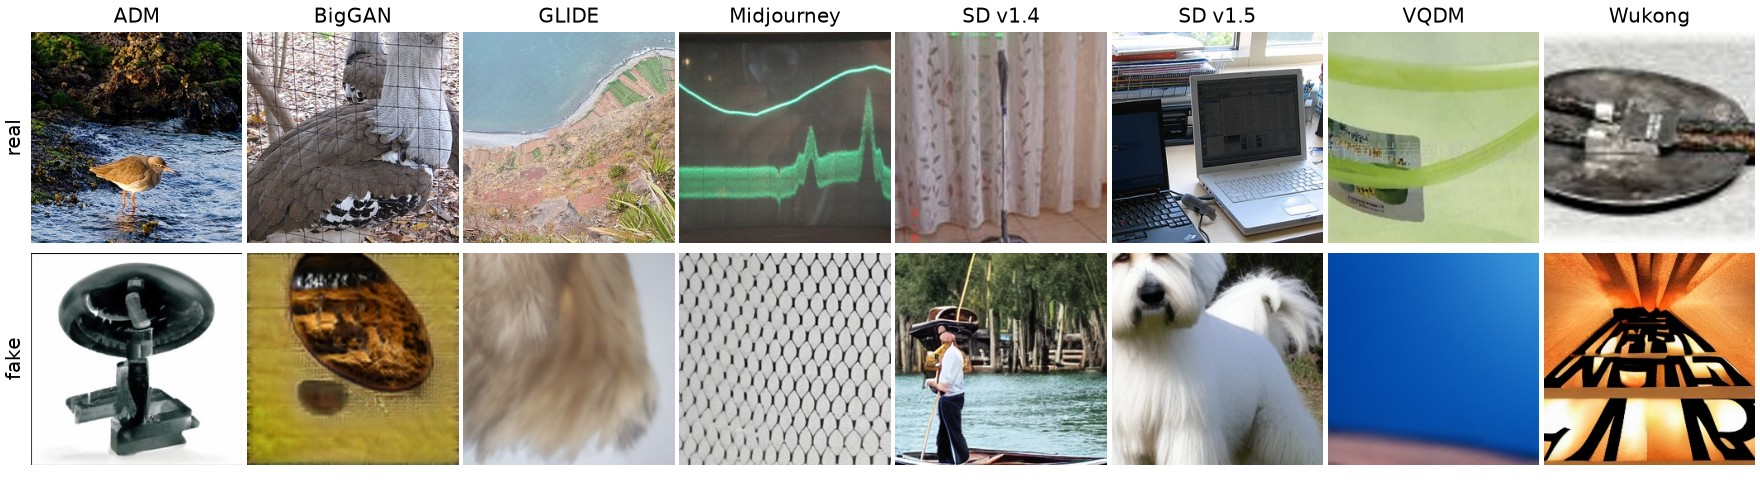
\includegraphics[width=\linewidth]{figures/examples.jpg}
\caption{One real (top) and one fake (bottom) image per generator after preprocessing, drawn at random from \texttt{meta\_val} with a fixed seed.}
\label{fig:examples}
\end{figure}

This does not remove every confound. Only 8.7\% of real images had a short side below 256\,px and were upscaled, but all BigGAN fakes ($128\times128$) were, while no other generator's fakes were. A linear probe on CLIP features, trained on real images only to separate upscaled from non-upscaled images, reaches an AUROC (defined in Section~\ref{sec:protocol}) of 0.965 (0.95--0.98 per generator). A control that resamples the same images without changing their content confirms that CLIP detects the resampling itself (AUROC 0.907). The trace is therefore available to the experts, and for the BigGAN expert it coincides with the fake label, which may inflate its in-distribution score (validation AUROC 0.9999). It also reaches the experts' outputs: among real \texttt{meta\_val} images, the BigGAN expert calls 5.9\% of the upscaled ones fake against 0.4\% of the others with CLIP, and 1.9\% against 0.2\% with ResNet-50. The cue need not affect all combiners alike, because a combiner that sees expert identity can learn what a high BigGAN score means, while an identity-blind one cannot; identity-aware combiners are not better on any backbone, though (Section~\ref{sec:results}). As a held-out generator, BigGAN may become harder rather than easier, because the remaining experts only saw upscaled reals. This fits the ResNet-50 pool, where the best single expert does worst on the BigGAN fold, but not the CLIP pool. Cropping without resizing also means the crop covers a different share of each original image (half the width for SD and Wukong, a quarter for Midjourney).

Finally, every real image was a JPEG before our preprocessing, so after re-encoding it has been compressed twice, while a fake has been compressed once~\cite{grommelt2024fake}. An expert could learn ``compressed before'' instead of the traces of its generator. We test this by giving fakes the same history. For each generator we take 500 fake and 500 real \texttt{meta\_val} images, compress the fakes once more at JPEG quality 90 or 75 before the usual quality-95 re-encoding, leave the reals untouched, and score all of them with the generator's own ResNet-50 expert (Section~\ref{sec:resnet}). Without the extra pass the experts call 96.8--100\% of fakes fake at a logit threshold of zero, while calling 0.2--2.8\% of reals fake. After it, this falls to 61.6--93.8\% at quality 90 and to 23.2--74.6\% at quality 75. The ranking holds up much better: AUROC stays at 0.950 or above at quality 90 and 0.916 or above at quality 75. Compression history therefore moves the experts' decisions a great deal, but it is not the main thing they rank on. The check cannot fully separate the two explanations, because a strong JPEG pass also erases part of the generator's own high-frequency traces, so a shortcut and damaged evidence predict the same drop. In practice, the decision threshold is the fragile part of such a detector, and it would need to be re-fitted for images with an unknown compression history.

\section{Experts}\label{sec:experts}

We use PyTorch~\cite{paszke2019pytorch} and torchvision for the ResNets, Hugging Face Transformers~\cite{wolf2020transformers} for CLIP, scikit-learn~\cite{pedregosa2011sklearn} for the logistic regressions and nearest neighbours, and NumPy~\cite{harris2020numpy} and pandas~\cite{mckinney2010pandas} for the analysis. We build on two sets of pretrained weights, OpenAI's CLIP ViT-L/14 and torchvision's ImageNet ResNet-50.

An expert is a binary classifier that separates real images from the fakes of a single generator family. It is trained only on that family's real and fake images (\texttt{expert\_train}) and validated on \texttt{expert\_val}. We train seven experts per backbone, one each for ADM, BigGAN, GLIDE, Midjourney, Stable Diffusion, VQDM and Wukong. Stable Diffusion v1.4 and v1.5 produce near-identical images, so they share one expert, whose training data is drawn half from each version; every expert therefore sees the same number of images (10,000 for training, 2,000 for validation).

We build two pools of experts on exactly the same images: linear probes on frozen CLIP features (Section~\ref{sec:clip}) and fine-tuned ResNets (Section~\ref{sec:resnet}), which lets us compare the two expert types (RQ4). Every expert outputs one raw logit per image. These logits are the input to the meta-learners in Section~\ref{sec:meta}.

\subsection{CLIP experts}\label{sec:clip}

\subsubsection{Background: CLIP}\label{sec:clip-background}

CLIP~\cite{radford2021clip} learns visual features from natural language instead of fixed class labels. An image encoder and a text encoder are trained together to predict which caption belongs to which image within a batch, using about 400 million image--text pairs collected from the internet. CLIP is therefore never trained to separate real from generated images. Each encoder's output is mapped by a linear projection into a shared embedding space in which matching images and captions lie close together. We use this projected image embedding, a 768-dimensional vector, as the feature for our experts. Of the image encoders trained by Radford et al., we use the Vision Transformer ViT-L/14~\cite{dosovitskiy2021vit} with the weights released by OpenAI\footnote{\texttt{openai/clip-vit-large-patch14} on the Hugging Face Hub.} at 224\,px input resolution, with all weights frozen.

Our CLIP experts follow the recipe of Ojha et al.~\cite{ojha2023universal}, a linear classifier on frozen CLIP ViT-L/14 features, which generalises to unseen generators much better than detectors trained for the task (Section~\ref{sec:intro}). Unlike them, we train one linear probe per generator family rather than a single probe.

\subsubsection{From features to experts}

\paragraph{Features.}
The embedding is computed once per image and stored. As input we use a $224\times224$ center crop of the $256\times256$ image, normalised with CLIP's mean and standard deviation; we deliberately do not use CLIP's standard preprocessing, which resizes the image first and would blur the pixel-level traces we preserve in Section~\ref{sec:preprocessing}.

\paragraph{Choice of classifier.}
A linear probe beats $k$-nearest neighbours under cosine distance, the other head used by Ojha et al.~\cite{ojha2023universal}, by 11.8 accuracy points on the expert's own generator and 2.5 points on the others (Appendix~\ref{app:knn}), so we use it as the expert head.

\paragraph{The seven experts.}
Each CLIP expert standardises the features and fits a logistic regression with the default L2 regularisation ($C=1$), identical for all experts and not tuned. Accuracy varies by at most 1.1 points for $C$ between 0.01 and 10, so this choice is not critical; as $C$ was compared on validation images, we treat this as a sensitivity check rather than tuning. All seven experts reach a validation AUROC of at least 0.986 (accuracy 0.942--0.995); the diagonal of Table~\ref{tab:cross-auroc} in Section~\ref{sec:pools} shows the same on \texttt{meta\_val}. The BigGAN expert's near-perfect score (AUROC 0.9999) may be inflated by the upscaling cue discussed in Section~\ref{sec:preprocessing}. As scores we use the raw logits of the logistic regression.

\subsection{ResNet experts}\label{sec:resnet}

The CLIP experts add a single linear layer to features that were never trained for detection. The ResNet experts are the opposite case: every weight is adapted to one generator. We use ResNet-50~\cite{he2016resnet}, the network GenImage uses for its own cross-generator experiments, where it reaches near-perfect accuracy on the training generator and weak transfer to the rest~\cite{zhu2023genimage}.

\paragraph{Model and training.}
Each expert starts from torchvision's ImageNet-pretrained weights, with its classifier replaced by a single logit. All layers are fine-tuned on the expert's \texttt{expert\_train} images with binary cross-entropy and AdamW~\cite{loshchilov2019adamw} (weight decay $10^{-4}$), using a one-cycle schedule with a peak learning rate of $10^{-4}$, batches of 64 and at most 8 epochs. As input we use $224\times224$ crops of the $256\times256$ images, the resolution of the pretrained weights: random crops with horizontal flips for training, the center crop for evaluation. Cropping instead of resizing leaves the pixel-level traces of Section~\ref{sec:preprocessing} intact. We keep the epoch with the lowest loss on \texttt{expert\_val} and stop after two epochs without improvement. We select on loss rather than accuracy or AUROC because both saturate early and then barely separate one epoch from the next, while the loss still does.

\paragraph{Temperature.}
Since deep networks are often overconfident~\cite{guo2017calibration}, we also fit a temperature $T \geq 1$ per expert on \texttt{expert\_val}. It stays between 1.00 and 1.12 (Appendix~\ref{app:resnet}), so the experts need almost no correction on their own generator. Like the CLIP experts, they pass on raw logits; a temperature would not change an expert's AUROC anyway.

\paragraph{Scores and cost.}
All seven experts reach a validation AUROC of at least 0.996. As with the CLIP BigGAN expert, the perfect BigGAN score may be inflated by the upscaling cue (Section~\ref{sec:preprocessing}). Each expert scores all 96{,}000 images outside \texttt{expert\_train}, giving seven logits per image and pool. Each expert was trained once, so we cannot report variation between seeds. On a single Apple M4 laptop, training the seven experts took 3.6\,h (20 to 45 minutes each) and scoring all images about 1.5\,h.

\paragraph{A smaller backup pool.}
Because ResNet-50 training is slow on a laptop, we first trained a ResNet-18 pool with the identical recipe as a fallback, in 50 minutes for all seven experts. We keep it only as a check on the main results. On its own generators it is close to ResNet-50 (validation AUROC 0.988 or above), but it transfers worse (Section~\ref{sec:pools}), and all seven experts need a temperature above 1 (1.06 to 1.43), while ResNet-50 needed almost none.

\subsection{Comparison of the expert pools}\label{sec:pools}

Table~\ref{tab:cross-auroc} shows the AUROC of every expert on every generator's \texttt{meta\_val} images. On their own generators the pools are close: at least 0.990 for CLIP and 0.995 for ResNet-50. They differ in transfer. Over the 48 cells where an expert meets a generator it was not trained on, the mean AUROC is 0.892 for CLIP and 0.794 for ResNet-50. CLIP is higher in 41 of these cells, and only 1 CLIP cell falls below 0.7, against 11 for ResNet-50. This agrees with the finding of Ojha et al.~\cite{ojha2023universal} that frozen CLIP features transfer better than detectors trained for the task. The smaller ResNet-18 backup pool (Section~\ref{sec:resnet}, not shown) falls further behind: 0.751 mean transfer AUROC, with 17 cells below 0.7. On the generators they were trained on the pools are almost indistinguishable; they separate only once the generator changes, which is exactly where the combiners have to work.

The seven cells where ResNet-50 is higher are ADM to BigGAN, GLIDE and Midjourney, Stable Diffusion to GLIDE and Wukong, and Wukong to both Stable Diffusion versions. ResNet transfer can therefore be strong, but it is narrow. Stable Diffusion and Wukong detect each other at 0.992 or above, while the BigGAN expert is close to chance on both (0.536 to 0.573). The Midjourney expert falls below chance on BigGAN (0.437), scoring BigGAN fakes as more real than real images. The BigGAN expert has the lowest mean transfer in both pools (0.649 for ResNet-50, 0.817 for CLIP). A low score in one expert is usually offset by another: for every generator, some other expert reaches at least 0.890 with ResNet-50 and 0.947 with CLIP, which leaves room for a combiner to help.

\begin{table}[t]
\centering
\small
\setlength{\tabcolsep}{4pt}
\begin{tabular}{lcccccccc}
\toprule
Expert & ADM & BigGAN & GLIDE & MJ & SD 1.4 & SD 1.5 & VQDM & Wukong \\
\midrule
\multicolumn{9}{l}{\textit{CLIP linear probes}} \\
ADM    & \textbf{.992} & .954 & .976 & .781 & .906 & .890 & .973 & .862 \\
BigGAN & .862 & \textbf{1.000} & .991 & .723 & .777 & .790 & .899 & .677 \\
GLIDE  & .916 & .992 & \textbf{.998} & .799 & .875 & .884 & .904 & .810 \\
MJ     & .755 & .777 & .854 & \textbf{.990} & .966 & .963 & .782 & .936 \\
SD     & .876 & .840 & .911 & .947 & \textbf{.993} & \textbf{.992} & .927 & .974 \\
VQDM   & .967 & .977 & .962 & .866 & .932 & .919 & \textbf{.992} & .916 \\
Wukong & .871 & .879 & .924 & .935 & .989 & .988 & .927 & \textbf{.991} \\
\midrule
\multicolumn{9}{l}{\textit{ResNet-50}} \\
ADM    & \textbf{.997} & .967 & .994 & .821 & .784 & .791 & .950 & .741 \\
BigGAN & .673 & \textbf{1.000} & .946 & .638 & .546 & .573 & .630 & .536 \\
GLIDE  & .873 & .899 & \textbf{1.000} & .732 & .820 & .812 & .769 & .744 \\
MJ     & .684 & .437 & .773 & \textbf{.995} & .930 & .940 & .562 & .900 \\
SD     & .788 & .670 & .923 & .945 & \textbf{.999} & \textbf{1.000} & .792 & .992 \\
VQDM   & .890 & .782 & .937 & .769 & .754 & .724 & \textbf{.998} & .718 \\
Wukong & .731 & .692 & .838 & .899 & .997 & .998 & .821 & \textbf{.999} \\
\bottomrule
\end{tabular}
\caption{AUROC of each expert (rows) on each generator's \texttt{meta\_val} images (columns). Bold marks the expert's own generator(s). The \texttt{test} pool was not used.}
\label{tab:cross-auroc}
\end{table}

\subsection{Generalists}\label{sec:generalists}

The obvious alternative to combining experts is not to split the data in the first place. For every leave-one-out fold we therefore also train one \emph{generalist} per backbone on the \texttt{expert\_train} images of all known generators together: the union of the training sets of the remaining experts, 60,000 images (50,000 when Stable Diffusion and Wukong are held out together). The generalist sees exactly the images the experts see between them, so the comparison asks one question only: one model, or several models and a combiner? If anything it favours the combiners, which are additionally fitted on \texttt{meta\_train}, images the generalist never sees.

The CLIP generalist is the expert recipe unchanged, a logistic regression with $C=1$ on standardised CLIP features. The ResNet-50 generalist uses the expert recipe as well, with early stopping and the temperature fitted on the \texttt{expert\_val} images of the known generators. We train eight ResNet-50 generalists, one for each of the seven single-family folds and one that holds out Stable Diffusion (v1.4 and v1.5) and Wukong together; the main evaluation uses six of them (Section~\ref{sec:protocol}). On the known generators all eight reach a validation AUROC of 0.998 or 0.999, with the best epoch between 4 and 8. Unlike the ResNet-50 experts, every generalist needs a clear temperature correction ($T$ between 1.22 and 1.61): a single network covering six generators is overconfident even on images from those generators. Each generalist took 95 to 136 minutes to train, about 16\,h in total, between four and five times the cost of the seven ResNet-50 experts. Generalists are evaluated exactly like a meta-learner: the decision threshold comes from the known generators' \texttt{meta\_val} images, and AUROC, AP and accuracy are measured on the held-out generator only. On the held-out generators the ResNet-50 generalists reach a mean AUROC of 0.978, from 0.965 for ADM to 0.999 for GLIDE, against 0.999 on the known generators (Appendix~\ref{app:generalists}). The ranking therefore transfers well, but the threshold transfers less well: accuracy falls to 84.2\% on average and to about 76\% for ADM and BigGAN.

\section{Meta-learners}\label{sec:meta}

A meta-learner (or combiner) takes the raw logits produced by the active experts for a given image and outputs a single real-versus-fake score. We organize our candidate combiners along two axes (Figure~\ref{fig:overview}b): \emph{identity-awareness} and \emph{flexibility}. This structure allows us to isolate whether transfer to unseen generators fails because a combiner overfits due to excess capacity (RQ3), or because it relies on expert identities that no longer apply (RQ2).

\begin{figure}[t]
\centering
\resizebox{\textwidth}{!}{%
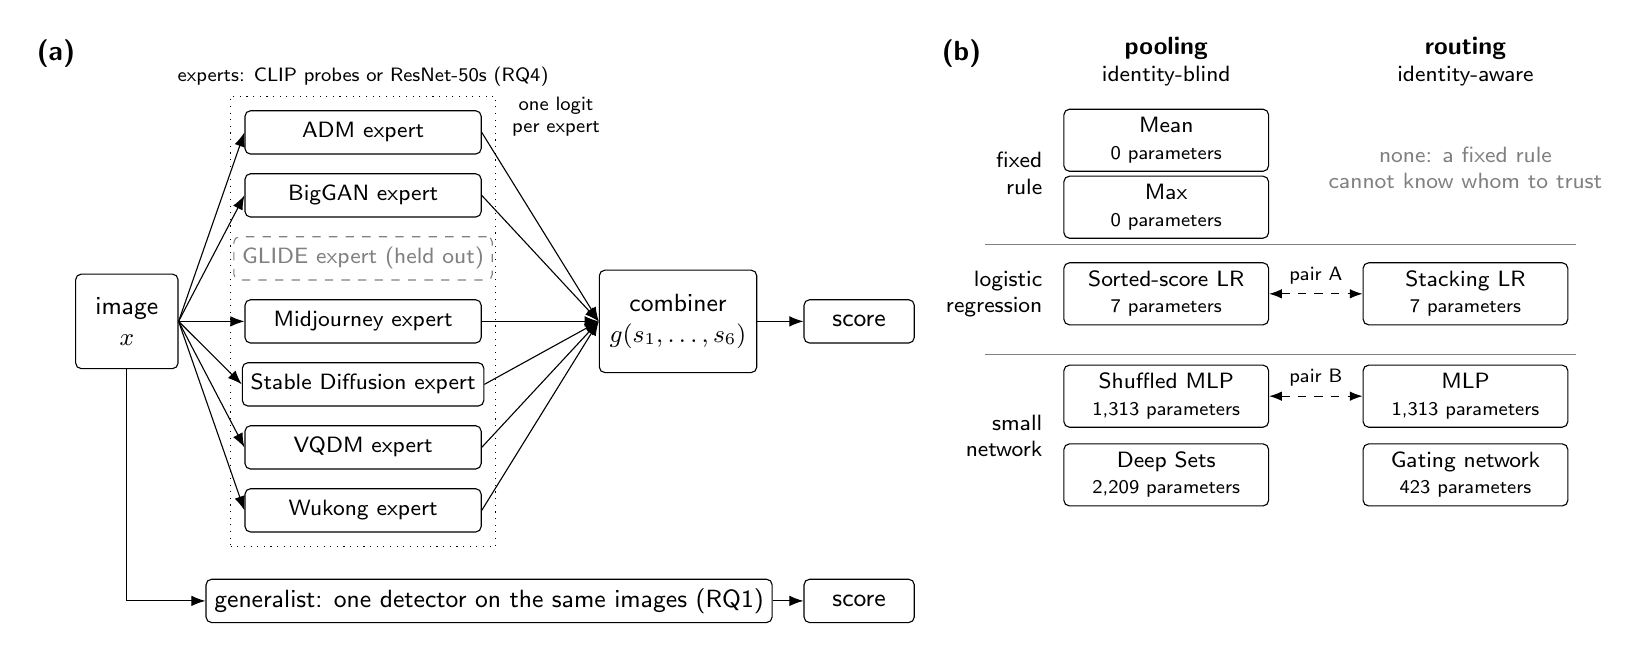
\begin{tikzpicture}[
  font=\sffamily\small,
  box/.style={draw, rounded corners=2pt, align=center, inner sep=3pt, minimum height=0.55cm},
  expert/.style={box, minimum width=3.0cm, font=\sffamily\footnotesize},
  method/.style={box, minimum width=2.6cm, minimum height=0.72cm, font=\sffamily\footnotesize},
  arr/.style={-{Latex[length=1.8mm]}},
]
% ---------------- (a) pipeline ----------------
\node[font=\sffamily\bfseries] at (-0.9,3.4) {(a)};
\node[box, minimum width=1.3cm, minimum height=1.2cm] (img) at (0,0) {image\\$x$};
\node[expert] (e1) at (3.0,2.4)  {ADM expert};
\node[expert] (e2) at (3.0,1.6)  {BigGAN expert};
\node[expert, dashed, text=gray, draw=gray] (e3) at (3.0,0.8) {GLIDE expert (held out)};
\node[expert] (e4) at (3.0,0.0)  {Midjourney expert};
\node[expert] (e5) at (3.0,-0.8) {Stable Diffusion expert};
\node[expert] (e6) at (3.0,-1.6) {VQDM expert};
\node[expert] (e7) at (3.0,-2.4) {Wukong expert};
\node[draw, dotted, fit=(e1)(e7), inner sep=5pt,
      label={[font=\sffamily\scriptsize]above:experts: CLIP probes or ResNet-50s (RQ4)}] {};
\node[box, minimum width=2.0cm, minimum height=1.3cm] (comb) at (7.0,0) {combiner\\$g(s_1,\dots,s_6)$};
\node[box, minimum width=1.4cm] (out) at (9.3,0) {score};
\foreach \e in {e1,e2,e4,e5,e6,e7} {
  \draw[arr] (img.east) -- (\e.west);
  \draw[arr] (\e.east) -- (comb.west);
}
\node[font=\sffamily\scriptsize, align=center] at (5.45,2.6) {one logit\\per expert};
\draw[arr] (comb) -- (out);
\node[box, minimum width=5.6cm] (gen) at (4.6,-3.55) {generalist: one detector on the same images (RQ1)};
\node[box, minimum width=1.4cm] (out2) at (9.3,-3.55) {score};
\draw[arr] (img.south) |- (gen.west);
\draw[arr] (gen) -- (out2);
% ---------------- (b) combiners ----------------
\node[font=\sffamily\bfseries] at (10.6,3.4) {(b)};
\node[font=\sffamily\small\bfseries, align=center] at (13.2,3.3) {pooling\\[-1pt]{\footnotesize\mdseries identity-blind}};
\node[font=\sffamily\small\bfseries, align=center] at (17.0,3.3) {routing\\[-1pt]{\footnotesize\mdseries identity-aware}};
\node[font=\sffamily\footnotesize, anchor=east, align=right] at (11.75,1.88)  {fixed\\rule};
\node[font=\sffamily\footnotesize, anchor=east, align=right] at (11.75,0.35) {logistic\\regression};
\node[font=\sffamily\footnotesize, anchor=east, align=right] at (11.75,-1.45) {small\\network};
\draw[gray] (10.9,0.98) -- (18.4,0.98);
\draw[gray] (10.9,-0.42) -- (18.4,-0.42);
\node[method] (mean) at (13.2,2.3) {Mean\\{\scriptsize 0 parameters}};
\node[method] (max)  at (13.2,1.45) {Max\\{\scriptsize 0 parameters}};
\node[font=\sffamily\footnotesize, text=gray, align=center] at (17.0,1.95) {none: a fixed rule\\cannot know whom to trust};
\node[method] (sort)  at (13.2,0.35) {Sorted-score LR\\{\scriptsize 7 parameters}};
\node[method] (stack) at (17.0,0.35) {Stacking LR\\{\scriptsize 7 parameters}};
\node[method] (shuf)  at (13.2,-0.95) {Shuffled MLP\\{\scriptsize 1,313 parameters}};
\node[method] (mlp)   at (17.0,-0.95) {MLP\\{\scriptsize 1,313 parameters}};
\node[method] (ds)    at (13.2,-1.95) {Deep Sets\\{\scriptsize 2,209 parameters}};
\node[method] (gate)  at (17.0,-1.95) {Gating network\\{\scriptsize 423 parameters}};
\draw[{Latex[length=1.6mm]}-{Latex[length=1.6mm]}, dashed] (sort) -- node[above, font=\sffamily\scriptsize] {pair A} (stack);
\draw[{Latex[length=1.6mm]}-{Latex[length=1.6mm]}, dashed] (shuf) -- node[above, font=\sffamily\scriptsize] {pair B} (mlp);
\end{tikzpicture}}
\caption{(a) Leave-one-generator-out setup, here with GLIDE held out: the held-out generator's expert is removed, the six remaining experts each give one logit, and a combiner turns them into one score. The generalist is the alternative: one detector trained on the images of all known generators. (b) The eight combiners by flexibility (rows) and identity-awareness (columns), with their trainable parameters for six experts (from our code). Each matched pair differs only in whether it sees which expert produced which logit.}
\label{fig:overview}
\end{figure}

\subsection{Pooling vs.\ Routing}

\textbf{Pooling} (identity-blind) combiners see only the pattern of scores, not which expert produced which, so we expect them to transfer more reliably to truly new generators. \textbf{Routing} (identity-aware) combiners know each expert's identity and learn whom to trust, so we expect them to do best on known generators and on held-out generators with a known ``sibling'' (such as Stable Diffusion and Wukong), and to drop more sharply on unrelated ones.

\subsection{Candidate Combiners}

We evaluate eight combiners spanning three levels of model capacity, alongside three reference points: the generalist from Section~\ref{sec:generalists}; the \emph{best expert}, the remaining expert with the highest AUROC on the known generators' \texttt{meta\_val} images, which is what one would deploy without a combiner; and the \emph{best expert in hindsight}, the remaining expert with the highest AUROC on the held-out generator itself, an upper bound for any rule that picks a single expert.

\paragraph{Fixed rules (0 parameters).}
The \textbf{Mean} combiner averages the logits of all available experts, serving as our simplest unweighted baseline. The \textbf{Max} combiner takes the highest logit, so an image counts as fake as soon as one expert is confident (a hard noisy-OR), reflecting the intuition that a novel generator may trigger only one specialist.

\paragraph{Linear models (low capacity).}
Standard \textbf{Logistic regression (stacking)} learns one weight per expert, capturing global trust preferences (e.g., weighting ADM higher than BigGAN). To separate linear capacity from identity-awareness, \textbf{Sorted-score LR} (Matched Pair A) sorts each image's expert logits from highest to lowest before applying logistic regression; it learns how much the strongest signals matter without knowing which experts produced them.

\paragraph{Neural networks (high capacity).}
A standard \textbf{MLP} takes the fixed-order vector of expert logits, allowing it to model non-linear interactions across experts (e.g., firing only when two specific specialists agree). Its identity-blind counterpart, the \textbf{Shuffled MLP} (Matched Pair B), uses the identical architecture and parameter count but shuffles the order of the logits independently for every training image, so no input position can stand for a particular expert; at prediction it averages over ten random orders. \textbf{Deep Sets}~\cite{zaheer2017deepsets} treat the experts' logits as an unordered set. A small network $\phi$ maps each logit on its own to a 32-dimensional vector, the vectors are summed over experts, and a second network $\rho$ maps the sum to the final score, $f(s_1,\dots,s_n) = \rho\big(\sum_i \phi(s_i)\big)$. Because a sum does not depend on the order of its terms, the output cannot depend on which expert produced which logit, and the same network accepts any number of experts. Unlike the sorted LR, it can still learn non-linear rules such as ``two confident experts count for more than one very confident expert''. Finally, a \textbf{Gating network (mixture of experts)} maps the vector of logits through a small network to one softmax weight per expert and outputs the weighted sum of the logits. Because each input position belongs to a fixed expert, it can learn per image which expert to trust, which makes it the most explicit form of routing.

\paragraph{Ablation: pseudo-unseen training.}\label{sec:pseudo}
As a diagnostic, not a separate method, we also train stacking LR, the MLP, Deep Sets and the gating network in a \emph{pseudo-unseen} (PU) variant. During fitting, each image's own expert, which recognises it almost perfectly, is hidden by setting its logit to 0 (for real images too, so hiding says nothing about the label); at prediction each expert is hidden in turn and the scores are averaged. If a combiner leans on the image's own expert, a shortcut that does not exist for an unseen generator, PU training should change it.


\subsection{Training details}\label{sec:training}

Both logistic regressions use $C=1$ on raw logits. The MLP has two hidden layers of 32 units with ReLU, and the shuffled MLP is identical; Deep Sets uses two layers of 32 units for both $\phi$ and $\rho$; the gate has one hidden layer of 32 units. All neural combiners are trained with binary cross-entropy and AdamW (learning rate $10^{-2}$, weight decay $10^{-4}$, batches of 256) for 20 epochs, keeping the epoch with the lowest loss on the known generators' \texttt{meta\_val} images, with three seeds (4001--4003); we report the mean over seeds. The standard deviation of mean AUROC over seeds is at most 0.001 for every neural combiner on CLIP and ResNet-50, except PU gating on CLIP (0.003). Standardising each expert's logits first changed mean AUROC by less than 0.004 for all combiners except the gating network and its PU variant, which it made worse (gating: 0.949 to 0.901 on ResNet-50), so combiners see raw logits.

\subsection{Evaluation protocol}\label{sec:protocol}

\paragraph{Folds.} Each fold holds out one generator family: its expert is removed, and its images are excluded from fitting and early stopping. Stable Diffusion and Wukong detect each other at AUROC 0.97 or above in both pools (Table~\ref{tab:cross-auroc}), so holding out one of them while the other's expert stays would not test an unseen generator. We therefore hold them out together, which gives six folds: ADM, BigGAN, GLIDE, Midjourney, VQDM, and Stable Diffusion (v1.4 and v1.5) with Wukong. The effect is not small: with seven folds, the ResNet-50 mean combiner would score 0.952 instead of 0.937. In each fold a combiner is fitted on the \texttt{meta\_train} images of the known generators (28,000 images, 20,000 in the joint fold), with six experts as input (five in the joint fold), and evaluated on the held-out generator's \texttt{test} images (4,000 per generator, 12,000 in the joint fold). We report the mean over folds.

\paragraph{Metrics.} \textbf{AUROC}, the area under the ROC curve, measures how well a score ranks fakes above reals: it is the probability that a randomly chosen fake image gets a higher score than a randomly chosen real one, so 0.5 is chance and 1 is perfect. It needs no decision threshold, which makes it our main metric for unseen generators. \textbf{AP} (average precision) is the area under the precision--recall curve with fakes as the positive class; for CLIP and ResNet-50 it stays within 0.01 of AUROC for every method, so we report AUROC. \textbf{Accuracy} needs a threshold, and a deployed detector cannot tune it on a generator it has never seen, so we choose the threshold with the highest accuracy on the known generators' \texttt{meta\_val} images and apply it unchanged to the held-out generator. \textbf{Known AUROC} is measured on the \texttt{test} images of the known generators, and the \textbf{gap} is known minus unseen AUROC, the measure of RQ3.

\paragraph{Use of the test pool.} All design choices (six folds, raw logits, combiner settings, the comparisons below) were made on \texttt{meta\_val}, and the \texttt{test} pool was evaluated once, after they were fixed. For CLIP and ResNet-50, every bootstrap conclusion on \texttt{test} is the same as on \texttt{meta\_val}, except two differences below 0.002 on CLIP (gating vs mean, PU Deep Sets vs Deep Sets), which switch between clear and not clear.

\subsection{Is a difference real? Paired bootstrap}\label{sec:bootstrap}

Seeds only cover the combiners' random initialisation; the test images are a random sample too. For every comparison we therefore run a paired bootstrap over the held-out images~\cite{efron1993bootstrap}. In each of 1,000 resamples we redraw, within every fold, the held-out real and fake images with replacement, keeping the fold's size and balance, and recompute the mean unseen AUROC over folds for \emph{both} methods on the same redrawn images. The 2.5th and 97.5th percentiles of the difference give a 95\% interval, and we call a difference \emph{clear} when this interval excludes zero. The comparisons were fixed before the \texttt{test} run.\footnote{Except the four comparisons of the ResNet generalists, added after the \texttt{test} run once their per-image scores were available; they mirror the CLIP generalist comparisons fixed in advance.} The bootstrap does not cover the training randomness of the experts, each trained once, nor the choice of generators: a claim about generators in general rests on six cases, which is why we also report every fold (Table~\ref{tab:folds}).

\section{Results}\label{sec:results}

Table~\ref{tab:main} gives the main results, Table~\ref{tab:bootstrap} the bootstrap intervals for the key comparisons behind each research question, and Table~\ref{tab:folds} the individual folds.

\begin{table}[t]
\centering
\small
\setlength{\tabcolsep}{5pt}
\begin{tabular}{llcccccc}
\toprule
 & & \multicolumn{3}{c}{CLIP} & \multicolumn{3}{c}{ResNet-50} \\
\cmidrule(lr){3-5}\cmidrule(lr){6-8}
Method & Type & AUROC & Acc. & Gap & AUROC & Acc. & Gap \\
\midrule
Best expert in hindsight (upper bound) & -- & .974 & -- & -- & .948 & -- & -- \\
Best expert (chosen on known) & -- & .908 & .818 & .039 & .806 & .695 & .107 \\
\midrule
Mean & P & .969 & .902 & .016 & .937 & .807 & .053 \\
Max & P & .966 & .886 & .024 & .946 & .756 & .052 \\
Sorted LR & P & .972 & .898 & .020 & .948 & .771 & .049 \\
Stacking LR & R & .970 & .903 & .016 & .944 & .810 & .048 \\
Shuffled MLP & P & .972 & .898 & .020 & .950 & .768 & .047 \\
MLP & R & .972 & .898 & .020 & .948 & .765 & .049 \\
Deep Sets & P & .972 & .899 & .019 & .949 & .777 & .048 \\
Gating & R & .969 & .897 & .021 & .949 & .768 & .048 \\
\midrule
Generalist & -- & \textbf{.975} & \textbf{.907} & \textbf{.016} & \textbf{.978} & \textbf{.842} & \textbf{.021} \\
\bottomrule
\end{tabular}
\caption{Unseen-generator results on \texttt{test}, mean over six folds (and three seeds for neural combiners). Type: P = pooling (identity-blind), R = routing (identity-aware). Accuracy uses the threshold fitted on the known generators; Gap = known minus unseen AUROC (lower is better). Bold: best per column. The pseudo-unseen ablation is in Appendix~\ref{app:pu}.}
\label{tab:main}
\end{table}

\begin{table}[t]
\centering
\small
\setlength{\tabcolsep}{4pt}
\begin{tabular}{llcc}
\toprule
RQ & Comparison (first minus second) & CLIP & ResNet-50 \\
\midrule
RQ1 & Mean $-$ best expert & $+$.0609 [.0583, .0637] & $+$.1309 [.1269, .1346] \\
    & Generalist $-$ MLP & $+$.0029 [.0018, .0039] & $+$.0303 [.0283, .0323] \\
\midrule
RQ2 & Stacking LR $-$ sorted LR & $-$.0013 [$-$.0022, $-$.0005] & $-$.0039 [$-$.0054, $-$.0024] \\
    & MLP $-$ shuffled MLP & $+$.0007 [.0002, .0012] & $-$.0018 [$-$.0024, $-$.0011] \\
\midrule
RQ3 & MLP $-$ mean & $+$.0032 [.0023, .0042] & $+$.0116 [.0099, .0133] \\
    & Gating $-$ mean & $+$.0002 [$-$.0009, .0012]$^\dagger$ & $+$.0125 [.0108, .0142] \\
\midrule
RQ4 & CLIP $-$ ResNet-50, mean & \multicolumn{2}{c}{$+$.0325 [.0297, .0354]} \\
\bottomrule
\end{tabular}
\caption{Paired bootstrap on \texttt{test}: difference in mean unseen AUROC with 95\% interval (1,000 resamples), one or two key comparisons per research question. All are clear except the one marked $^\dagger$. All 16 comparisons are in Appendix~\ref{app:bootstrap}.}
\label{tab:bootstrap}
\end{table}

\begin{table}[t]
\centering
\small
\setlength{\tabcolsep}{4pt}
\begin{tabular}{lcccccccc}
\toprule
 & \multicolumn{4}{c}{CLIP} & \multicolumn{4}{c}{ResNet-50} \\
\cmidrule(lr){2-5}\cmidrule(lr){6-9}
Held out & Hindsight & Mean & Deep Sets & Generalist & Hindsight & Mean & Deep Sets & Generalist \\
\midrule
ADM & .971 & .955 & .957 & .966 & .891 & .910 & .912 & .965 \\
BigGAN & .995 & .983 & .987 & .985 & .974 & .913 & .956 & .971 \\
GLIDE & .995 & .988 & .986 & .990 & .996 & .993 & .995 & .999 \\
Midjourney & .951 & .942 & .946 & .942 & .949 & .956 & .954 & .966 \\
VQDM & .976 & .981 & .983 & .988 & .962 & .926 & .955 & .989 \\
SD + Wukong & .957 & .966 & .972 & .979 & .919 & .921 & .925 & .981 \\
\bottomrule
\end{tabular}
\caption{Unseen AUROC per fold on \texttt{test}. Hindsight: the best single remaining expert on that generator, known only afterwards. Deep Sets stands for the strongest combiners, which differ by at most 0.003 on average.}
\label{tab:folds}
\end{table}

\paragraph{RQ1: Combining experts vs.\ individual experts and a single generalist.}
Combining helps a lot. Deploying the single expert that looks best on the known generators gives an unseen AUROC of 0.908 for CLIP and 0.806 for ResNet-50; even the plain mean of the experts reaches 0.969 and 0.937, and the best combiners 0.972 and 0.950 (Table~\ref{tab:main}). The gains are $+0.06$ for CLIP and $+0.13$ to $+0.14$ for ResNet-50, with intervals far from zero (Table~\ref{tab:bootstrap}; all comparisons in Appendix~\ref{app:bootstrap}). On average the combiners even match the best single expert in hindsight (0.950 vs 0.948 for ResNet-50), which no rule that picks one expert could do without knowing the answer. The generalist, however, beats every combiner on both backbones. For CLIP the margin is small ($+0.003$ to $+0.006$) and differs between folds: the generalist is ahead on three, level on GLIDE, and behind on BigGAN and Midjourney (Table~\ref{tab:folds}). For ResNet-50 it is large ($+0.029$ to $+0.042$) and holds on all six folds, reaching about $+0.05$ over the best combiner on ADM and on Stable Diffusion with Wukong. The answer to RQ1 is therefore yes compared with the individual experts, and no compared with one detector trained on all known generators.

\paragraph{RQ2: Routing by expert identity vs.\ identity-free pooling.}
Knowing which expert produced which score does not help. In both matched pairs the identity-blind partner is as good or better: the sorted LR beats stacking LR on both backbones ($-0.001$ and $-0.004$ for stacking), and the shuffled MLP beats the MLP on ResNet-50 ($-0.002$ for the MLP). The one difference in favour of identity, the MLP on CLIP, is $+0.0007$, an order of magnitude below the other effects in this study. The gating network, the most explicit router, is never better than Deep Sets. Section~\ref{sec:disc-identity} discusses why.

\paragraph{RQ3: Effect of combiner capacity on transfer.}
Capacity helps only when the experts are weak. On CLIP, the flexible combiners improve on the mean by at most 0.003, and the gating network not at all. On ResNet-50, the MLP, Deep Sets and gating network all gain about 0.012 over the mean, and stacking LR 0.008, all clear. The fixed rules already show why: on ResNet-50 the maximum beats the mean (0.946 vs 0.937), because a fake from an unseen generator often triggers only one or two experts and averaging dilutes them, whereas on CLIP, where most experts transfer, averaging wins (0.969 vs 0.966). The flexible combiners learn such rules from data. The overfitting does not appear in AUROC: on ResNet-50 the gap shrinks slightly with capacity (0.053 for the mean, 0.047--0.049 for the neural combiners), and on CLIP it grows only from 0.016 to about 0.020, because the flexible combiners fit the known generators better (known AUROC 0.991--0.992 vs 0.985 on CLIP, 0.997 vs 0.989 on ResNet-50) and the unseen ones about as much better. It appears in accuracy instead: on ResNet-50 the neural combiners lose 3 to 4 points against the mean (0.765--0.777 vs 0.807) despite their higher AUROC, because their threshold does not transfer (Section~\ref{sec:disc-threshold}).

\paragraph{RQ4: Dependence on the type of expert.}
The CLIP experts transfer better on their own (mean cross-generator AUROC 0.892 vs 0.794, Table~\ref{tab:cross-auroc}), and the advantage survives combination: CLIP combiners beat ResNet-50 combiners by $+0.024$ (MLP) to $+0.033$ (mean). What changes with the expert type is how much the combiner matters. With CLIP experts nearly every combiner lands between 0.966 and 0.972; with ResNet-50 experts combining gains twice as much over the best expert, and capacity adds another 0.012. For the generalists the ranking of the backbones reverses: the ResNet-50 generalist (0.978) is slightly ahead of the CLIP generalist (0.975). This comparison was not in our pre-fixed bootstrap list, so we report it as an observation. It suggests that the CLIP advantage belongs to experts that each see one generator, not to the backbone as such.

\paragraph{Ablation: pseudo-unseen training.}
Hiding each image's own expert does not improve ranking: the MLP loses 0.004 (CLIP) and 0.006 (ResNet-50) AUROC, and Deep Sets stays within 0.001. On ResNet-50 it does change the threshold of the two routing networks, raising the accuracy of the MLP from 0.765 to 0.815 and of the gating network from 0.768 to 0.814 (the level of the mean), while Deep Sets is unaffected (0.777; Appendix~\ref{app:pu}). This supports two of our explanations: routing combiners lean on the image's own expert (Section~\ref{sec:disc-identity}), and the transferred threshold, not the ranking, is what breaks (Section~\ref{sec:disc-threshold}).

\paragraph{ResNet-18 backup pool.}
The backup pool repeats the RQ1 and RQ4 findings (best expert 0.712, best combiner 0.891, generalist 0.933, all generalist margins clear). Its small RQ2 and RQ3 differences change sign between \texttt{meta\_val} and \texttt{test}, so we draw no conclusions from them.

\section{Discussion}\label{sec:discussion}

\subsection{Why one detector beats combined experts}\label{sec:disc-generalist}

For CLIP the answer is almost a matter of algebra. Every CLIP expert is an affine function of the same frozen 768-dimensional feature vector, so the mean of their logits, and any logistic regression on them, is again an affine classifier on those features, which is exactly the model class of the CLIP generalist. The linear combiners use no extra information. They estimate the same kind of classifier in a roundabout way, seven times on one generator each and then mixed, where the generalist estimates it once on all known generators. Accordingly, the margin is small and not consistent across folds.

For ResNet-50 the generalist also learns its own features, and here the margin is large and holds on every fold. The combiners reach about the level of the best single expert in hindsight (0.950 vs 0.948), so they seem to extract nearly all the information the expert scores contain. The limit is the scores themselves. Each expert compresses an image into one number that answers a narrow question: does this look like my generator? Traces shared by several generators, the ones most likely to appear in a new generator too, are not what any single expert is trained to report. The generalist is trained on the broader question, whether an image comes from \emph{any} known generator, and is therefore rewarded for exactly these shared traces. On five of the six folds it goes beyond the best single expert in hindsight; the exception is BigGAN, where one remaining expert alone already reaches 0.974. The generalist is not free, though: the eight ResNet-50 generalists took about 16\,h to train against 3.6\,h for the seven experts, and adding a generator means retraining, while a combiner needs one new expert and a refit that takes seconds. We did not test this incremental setting.

\subsection{Why expert identity does not help}\label{sec:disc-identity}

The best-expert baseline makes the difficulty concrete. Picking the expert that does best on the known generators gives 0.806 on ResNet-50, while the best expert in hindsight gives 0.948 (0.908 vs 0.974 on CLIP). Which expert to trust on a new generator cannot be read off the known generators, and that is precisely what routing has to do. Identity-aware combiners face the same problem in a softer form. On the known generators every image has an expert that recognises it almost perfectly, so the easiest rule to learn is to trust that expert when it fires; on the held-out generator no such expert exists. Identity-blind combiners can only learn rules about the pattern of scores, for example how strongly the most confident experts fire, and such rules do not depend on which generators happen to be known. It fits that pseudo-unseen training, which removes exactly this shortcut, raises the accuracy of the routing MLP and gating network on ResNet-50 by about 5 points and leaves that of Deep Sets unchanged.

\subsection{Ranking transfers, thresholds do not}\label{sec:disc-threshold}

Across the study, AUROC and accuracy tell different stories. The neural combiners on ResNet-50 rank unseen fakes better than the mean but classify them worse; the ResNet-50 generalist ranks at 0.978 but classifies only about 76\% of ADM and BigGAN images correctly; and in the JPEG check of Section~\ref{sec:preprocessing}, recompression barely moves the experts' AUROC but cuts the share of fakes they catch by up to three quarters. The mechanism is the same each time. A threshold fitted on the known generators sits where their fakes and the reals are far apart. Fakes from an unseen generator, or recompressed fakes, receive less extreme scores: still above the reals, but often below the threshold. The more sharply a model separates the known generators (known AUROC 0.997 for the neural combiners vs 0.989 for the mean on ResNet-50), the further the threshold moves away from where unseen fakes land. Pseudo-unseen training counters this by showing the combiner, during fitting, fakes that their own expert does not flag. For deployment, this suggests treating the threshold as something that must be re-fitted, or at least monitored, when the generator population changes.

\subsection{Limitations}

Our conclusions rest on six held-out generators from a single benchmark whose real images all come from ImageNet. The bootstrap covers the sampling of test images, not the choice of generators, and the experts were trained once each; the per-fold results (Table~\ref{tab:folds}) show which findings hold fold by fold (the ResNet-50 generalist margin) and which only on average (the CLIP generalist margin). We work with a 176,000-image subsample and $224\times224$ crops. Two dataset cues remain, the upscaling of small images and the double compression of reals (Section~\ref{sec:preprocessing}); our checks bound their effect but cannot remove it. Finally, the combiners only see one logit per expert; combiners that see the experts' internal features, or experts trained to report shared traces, might close part of the gap to the generalist.

\section{Conclusion}\label{sec:conclusion}

We asked whether combining generator-specific experts helps on a generator that none of them has seen. Three answers stand out. \textbf{First, combining clearly helps:} every combiner beats the best single expert, by 0.06 AUROC with CLIP experts and by 0.13 to 0.14 with ResNet-50 experts, and on average it matches the best expert one could only have picked in hindsight. \textbf{Second, how the experts are combined matters little:} ignoring which expert produced which score is never worse, and extra capacity only helps the weaker ResNet-50 experts, where it improves ranking but makes the decision threshold less reliable. \textbf{Third, one detector trained on all known generators is better still}, slightly with CLIP and clearly with ResNet-50. Our explanation is that an expert's score only says whether an image looks like its own generator, and so loses the traces that generators share. In practice, our results favour training one detector on all known generators and re-checking its threshold whenever new generators appear; combining experts pays off mainly where retraining that detector is too expensive.

\section*{AI Use Statement}
\addcontentsline{toc}{section}{AI Use Statement}
We used Claude (Anthropic) through Claude Code for coding, debugging and writing. It wrote or revised code for the ResNet experts, the evaluation of the generalists, the CLIP generalist, the best-expert baseline, pseudo-unseen training, the paired bootstrap and the JPEG check, and it drafted or edited parts of this report. \todo{Tim and Lída: add your tools and uses.} We reviewed and tested all generated code, recomputed every reported number from our saved results and checked every reference against its source. Our team chose the research questions, designed and ran all experiments on our own machines and interpreted the results.

\clearpage
\addcontentsline{toc}{section}{References}

\begin{thebibliography}{99}

\bibitem{deng2009imagenet}
Jia Deng, Wei Dong, Richard Socher, Li-Jia Li, Kai Li, and Li Fei-Fei.
ImageNet: A large-scale hierarchical image database.
In \emph{IEEE Conference on Computer Vision and Pattern Recognition (CVPR)}, pages 248--255, 2009.

\bibitem{dosovitskiy2021vit}
Alexey Dosovitskiy, Lucas Beyer, Alexander Kolesnikov, Dirk Weissenborn, Xiaohua Zhai, Thomas Unterthiner, Mostafa Dehghani, Matthias Minderer, Georg Heigold, Sylvain Gelly, Jakob Uszkoreit, and Neil Houlsby.
An image is worth 16x16 words: Transformers for image recognition at scale.
In \emph{International Conference on Learning Representations (ICLR)}, 2021.

\bibitem{efron1993bootstrap}
Bradley Efron and Robert J. Tibshirani.
\emph{An Introduction to the Bootstrap}.
Chapman \& Hall, 1993.

\bibitem{grommelt2024fake}
Patrick Grommelt, Louis Weiss, Franz-Josef Pfreundt, and Janis Keuper.
Fake or JPEG? Revealing common biases in generated image detection datasets.
\emph{arXiv preprint arXiv:2403.17608}, 2024.

\bibitem{guo2017calibration}
Chuan Guo, Geoff Pleiss, Yu Sun, and Kilian Q. Weinberger.
On calibration of modern neural networks.
In \emph{International Conference on Machine Learning (ICML)}, pages 1321--1330, 2017.

\bibitem{harris2020numpy}
Charles R. Harris, K. Jarrod Millman, St{\'e}fan J. van der Walt, et al.
Array programming with NumPy.
\emph{Nature}, 585(7825):357--362, 2020.

\bibitem{he2016resnet}
Kaiming He, Xiangyu Zhang, Shaoqing Ren, and Jian Sun.
Deep residual learning for image recognition.
In \emph{IEEE Conference on Computer Vision and Pattern Recognition (CVPR)}, pages 770--778, 2016.

\bibitem{jacobs1991adaptive}
Robert A. Jacobs, Michael I. Jordan, Steven J. Nowlan, and Geoffrey E. Hinton.
Adaptive mixtures of local experts.
\emph{Neural Computation}, 3(1):79--87, 1991.

\bibitem{loshchilov2019adamw}
Ilya Loshchilov and Frank Hutter.
Decoupled weight decay regularization.
In \emph{International Conference on Learning Representations (ICLR)}, 2019.

\bibitem{mckinney2010pandas}
Wes McKinney.
Data structures for statistical computing in Python.
In \emph{Proceedings of the 9th Python in Science Conference}, pages 56--61, 2010.

\bibitem{ojha2023universal}
Utkarsh Ojha, Yuheng Li, and Yong Jae Lee.
Towards universal fake image detectors that generalize across generative models.
In \emph{IEEE/CVF Conference on Computer Vision and Pattern Recognition (CVPR)}, pages 24480--24489, 2023.

\bibitem{paszke2019pytorch}
Adam Paszke, Sam Gross, Francisco Massa, et al.
PyTorch: An imperative style, high-performance deep learning library.
In \emph{Advances in Neural Information Processing Systems (NeurIPS)}, volume 32, 2019.

\bibitem{pedregosa2011sklearn}
Fabian Pedregosa, Ga{\"e}l Varoquaux, Alexandre Gramfort, et al.
Scikit-learn: Machine learning in Python.
\emph{Journal of Machine Learning Research}, 12:2825--2830, 2011.

\bibitem{radford2021clip}
Alec Radford, Jong Wook Kim, Chris Hallacy, Aditya Ramesh, Gabriel Goh, Sandhini Agarwal, Girish Sastry, Amanda Askell, Pamela Mishkin, Jack Clark, Gretchen Krueger, and Ilya Sutskever.
Learning transferable visual models from natural language supervision.
In \emph{International Conference on Machine Learning (ICML)}, pages 8748--8763, 2021.

\bibitem{wolf2020transformers}
Thomas Wolf, Lysandre Debut, Victor Sanh, et al.
Transformers: State-of-the-art natural language processing.
In \emph{Proceedings of the 2020 Conference on Empirical Methods in Natural Language Processing: System Demonstrations}, pages 38--45, 2020.

\bibitem{wolpert1992stacked}
David H. Wolpert.
Stacked generalization.
\emph{Neural Networks}, 5(2):241--259, 1992.

\bibitem{zaheer2017deepsets}
Manzil Zaheer, Satwik Kottur, Siamak Ravanbakhsh, Barnab{\'a}s P{\'o}czos, Ruslan Salakhutdinov, and Alexander J. Smola.
Deep sets.
In \emph{Advances in Neural Information Processing Systems (NeurIPS)}, pages 3391--3401, 2017.

\bibitem{zhu2023genimage}
Mingjian Zhu, Hanting Chen, Qiangyu Yan, Xudong Huang, Guanyu Lin, Wei Li, Zhijun Tu, Hailin Hu, Jie Hu, and Yunhe Wang.
GenImage: A million-scale benchmark for detecting AI-generated image.
In \emph{Advances in Neural Information Processing Systems (NeurIPS), Datasets and Benchmarks Track}, 2023.

\end{thebibliography}

\clearpage
\appendix
\addcontentsline{toc}{section}{Appendices}
\titleformat{\section}{\large\bfseries}{Appendix \thesection}{0.6em}{}

\section{Sampling of the shards}\label{app:sampling}
The Hugging Face mirror stores each generator's training split in shards of about 0.5\,GB, with rows sorted by ImageNet class. Reading shards in order would therefore cover only the first classes. Instead, we visit shards in a coarse-to-fine order ($0, n/2, n/4, 3n/4, n/8, \ldots$), so that the visited shards span the whole class range wherever sampling stops. We take at most 150 images per label per shard and assign each accepted image to a pool at random, weighted by how many images that pool still needs. Pools therefore fill evenly and mix images from many shards and classes. If a label is still short after this pass (e.g.\ BigGAN fakes, which sit in only a few shards), we revisit only the shards known to contain it.

\section{Linear probe vs.\ nearest neighbours}\label{app:knn}
As the classifier on top of the features we compare a linear probe (logistic regression) with $k$-nearest-neighbour classification under cosine distance, the two heads used by Ojha et al.~\cite{ojha2023universal}. For each expert, both are trained on its \texttt{expert\_train} images and evaluated by accuracy on the \texttt{expert\_val} images of all generators. In-distribution, the linear probe beats the best kNN setting ($k$ up to 999, uniform or distance-weighted votes) for every expert, by 9.4 to 14.5 percentage points (mean 11.8). On the other generators it wins on average (+2.5 points) and for five of the seven experts, but loses for BigGAN ($-10.1$) and GLIDE ($-4.6$). These two probes call most fakes from distant generators real; the BigGAN probe, for example, reaches only 0.51 accuracy on Stable Diffusion v1.4. Since nearest neighbours with our 10,000 training images per expert do not match the linear probe, we use the probe as the expert head.

\section{ResNet-50 expert training}\label{app:resnet}
\begin{table}[H]
\centering
\small
\begin{tabular}{lccccc}
\toprule
Expert & Best / last epoch & AUROC & Accuracy & Loss & $T$ \\
\midrule
ADM        & 2 / 4 & 0.9962 & 0.9730 & 0.0790 & 1.000 \\
BigGAN     & 4 / 6 & 1.0000 & 0.9985 & 0.0047 & 1.000 \\
GLIDE      & 7 / 8 & 0.9999 & 0.9965 & 0.0106 & 1.000 \\
Midjourney & 4 / 6 & 0.9977 & 0.9775 & 0.0587 & 1.068 \\
Stable Diffusion & 8 / 8 & 0.9991 & 0.9910 & 0.0354 & 1.122 \\
VQDM       & 3 / 5 & 0.9992 & 0.9870 & 0.0357 & 1.000 \\
Wukong     & 8 / 8 & 0.9992 & 0.9830 & 0.0367 & 1.000 \\
\bottomrule
\end{tabular}
\caption{ResNet-50 experts on \texttt{expert\_val} at the selected epoch, before temperature scaling.}
\label{tab:resnet-experts}
\end{table}

\section{ResNet-50 generalists per fold}\label{app:generalists}
\begin{table}[H]
\centering
\small
\begin{tabular}{lccccc}
\toprule
Held-out generator & AUROC & AP & Accuracy & Known AUROC & Gap \\
\midrule
ADM              & 0.9654 & 0.9669 & 0.7585 & 0.9996 & 0.0342 \\
BigGAN           & 0.9711 & 0.9672 & 0.7558 & 0.9991 & 0.0281 \\
GLIDE            & 0.9991 & 0.9991 & 0.9875 & 0.9991 & 0.0000 \\
Midjourney       & 0.9656 & 0.9677 & 0.8065 & 0.9989 & 0.0333 \\
VQDM             & 0.9886 & 0.9880 & 0.8725 & 0.9989 & 0.0103 \\
SD + Wukong      & 0.9808 & 0.9782 & 0.8689 & 0.9988 & 0.0180 \\
\midrule
Mean             & 0.9784 & 0.9779 & 0.8416 & 0.9991 & 0.0207 \\
\bottomrule
\end{tabular}
\caption{ResNet-50 generalists, one per leave-one-out fold, on the \texttt{test} pool. AUROC, AP and accuracy are measured on the held-out generator(s); accuracy uses the threshold fitted on the known generators' \texttt{meta\_val} images. Known AUROC is the AUROC on the \texttt{test} images of the known generators, and the gap is known minus held-out AUROC.}
\label{tab:generalists}
\end{table}

\section{All bootstrap comparisons}\label{app:bootstrap}
\begin{table}[H]
\centering
\small
\setlength{\tabcolsep}{4pt}
\begin{tabular}{llcc}
\toprule
RQ & Comparison (first minus second) & CLIP & ResNet-50 \\
\midrule
RQ1 & Mean $-$ best expert & $+$.0609 [.0583, .0637] & $+$.1309 [.1269, .1346] \\
    & MLP $-$ best expert & $+$.0641 [.0615, .0671] & $+$.1425 [.1379, .1466] \\
    & Generalist $-$ mean & $+$.0061 [.0051, .0069] & $+$.0419 [.0396, .0441] \\
    & Generalist $-$ sorted LR & $+$.0036 [.0026, .0046] & $+$.0302 [.0282, .0323] \\
    & Generalist $-$ MLP & $+$.0029 [.0018, .0039] & $+$.0303 [.0283, .0323] \\
    & Generalist $-$ Deep Sets & $+$.0032 [.0023, .0042] & $+$.0291 [.0271, .0311] \\
\midrule
RQ2 & Stacking LR $-$ sorted LR & $-$.0013 [$-$.0022, $-$.0005] & $-$.0039 [$-$.0054, $-$.0024] \\
    & MLP $-$ shuffled MLP & $+$.0007 [.0002, .0012] & $-$.0018 [$-$.0024, $-$.0011] \\
\midrule
RQ3 & Stacking LR $-$ mean & $+$.0012 [.0009, .0014] & $+$.0077 [.0067, .0087] \\
    & MLP $-$ mean & $+$.0032 [.0023, .0042] & $+$.0116 [.0099, .0133] \\
    & Deep Sets $-$ mean & $+$.0028 [.0020, .0036] & $+$.0128 [.0113, .0143] \\
    & Gating $-$ mean & $+$.0002 [$-$.0009, .0012]$^\dagger$ & $+$.0125 [.0108, .0142] \\
\midrule
RQ4 & CLIP $-$ ResNet-50, mean & \multicolumn{2}{c}{$+$.0325 [.0297, .0354]} \\
    & CLIP $-$ ResNet-50, MLP & \multicolumn{2}{c}{$+$.0241 [.0216, .0267]} \\
\midrule
Abl. & PU MLP $-$ MLP & $-$.0040 [$-$.0048, $-$.0033] & $-$.0063 [$-$.0076, $-$.0049] \\
    & PU Deep Sets $-$ Deep Sets & $+$.0004 [.0001, .0007] & $-$.0010 [$-$.0016, $-$.0004] \\
\bottomrule
\end{tabular}
\caption{Paired bootstrap on \texttt{test}: difference in mean unseen AUROC with 95\% interval (1,000 resamples). All differences are clear except the one marked $^\dagger$. Abl.: pseudo-unseen ablation.}
\label{tab:bootstrap-full}
\end{table}

\section{Pseudo-unseen ablation}\label{app:pu}
\begin{table}[H]
\centering
\small
\setlength{\tabcolsep}{5pt}
\begin{tabular}{llcccccc}
\toprule
 & & \multicolumn{3}{c}{CLIP} & \multicolumn{3}{c}{ResNet-50} \\
\cmidrule(lr){3-5}\cmidrule(lr){6-8}
Method & Type & AUROC & Acc. & Gap & AUROC & Acc. & Gap \\
\midrule
PU stacking LR & R & .969 & .902 & .016 & .944 & .812 & .047 \\
PU MLP & R & .968 & .890 & .019 & .942 & .815 & .047 \\
PU Deep Sets & P & .972 & .900 & .018 & .948 & .777 & .048 \\
PU gating & R & .963 & .879 & .020 & .942 & .814 & .047 \\
\bottomrule
\end{tabular}
\caption{Pseudo-unseen (PU) variants on \texttt{test}, same columns as Table~\ref{tab:main}, where the plain versions are listed.}
\label{tab:pu}
\end{table}

\end{document}
